\documentclass[11pt,letterpaper]{article}

% Essential packages
\usepackage[utf8]{inputenc}
\usepackage[T1]{fontenc}
\usepackage[margin=1in]{geometry}
\usepackage{fancyhdr}
\usepackage{graphicx}
\usepackage{float}

% Math packages
\usepackage{amsmath}
\usepackage{amsfonts}
\usepackage{amssymb}
\usepackage{amsthm}

% Table packages
\usepackage{booktabs}
\usepackage{array}
\usepackage{tabularx}
\usepackage{longtable}

% List packages
\usepackage{enumitem}
\usepackage{float}

% Graphics and plotting
\usepackage{tikz}
\usepackage{pgfplots}
\pgfplotsset{compat=1.18}
\usepackage{subcaption}

% Citation and references
\usepackage[round,authoryear]{natbib}
\usepackage{url}

% Code listings (if needed for simulation code)
\usepackage{listings}
\usepackage{xcolor}

% Hyperlinks (load last)
\usepackage[colorlinks=true,linkcolor=blue,citecolor=blue,urlcolor=blue]{hyperref}

% Custom commands for common actuarial notation
\newcommand{\E}{\mathbb{E}}
\newcommand{\Var}{\text{Var}}
\newcommand{\Cov}{\text{Cov}}
\newcommand{\Prob}{\mathbb{P}}

% Header and footer setup
\pagestyle{fancy}
\fancyhf{}
\fancyhead[L]{Ergodicity Simulation Framework for Insurance}
\fancyhead[R]{}
\fancyfoot[C]{\thepage}

% Title page information
\title{\Large \textbf{Ergodicity Economics in Property \& Casualty Insurance: \\
A Simulation Framework for Understanding Risk Appetite}}

\author{Alex Filiakov, ACAS\\
\texttt{alexfiliakov@gmail.com}}

\date{\today}

\begin{document}

\maketitle

\begin{abstract}
This white paper introduces a new simulation framework based on ergodicity economics principles for analyzing insurance risk appetite in Property \& Casualty markets. Traditional ensemble-based risk models may not adequately capture the temporal dynamics of insurance company decision-making. This introductory paper demonstrates that insurance appetite varies significantly with company size, measured by revenue.
\\\\
\textbf{Keywords:} ergodicity economics, insurance appetite, risk modeling, simulation framework
\end{abstract}

\newpage
\tableofcontents
\newpage

\section{Executive Summary}

This section should provide a concise overview of the entire paper, typically 1-2 pages covering:
\begin{itemize}
    \item The problem addressed
    \item Your key methodology (simulation framework)
    \item Primary finding about company size and insurance appetite
    \item Practical implications for the industry
\end{itemize}

% TODO: Complete executive summary content

\section{Introduction}

\subsection{Current Challenges in Insurance Appetite Modeling}

Traditional approaches to modeling insurance appetite in P\&C markets face several limitations:
\begin{itemize}
    \item Reliance on ensemble averages rather than temporal sequences
    \item Inadequate consideration of path-dependent effects
    \item Limited incorporation of company-specific factors
\end{itemize}

\subsection{The Promise of Ergodicity Economics}

Ergodicity economics, developed by \citet{peters2025ergodicity}, offers a new perspective on decision-making under uncertainty. Unlike traditional expected utility theory, which focuses on ensemble averages, ergodicity economics emphasizes the importance of time averages and growth rates.

% TODO: Add more detailed introduction content

\section{Theoretical Foundation}

\subsection{Ergodicity vs. Non-Ergodicity in Financial Systems}

A stochastic process is ergodic if its time average equals its ensemble average:
\begin{equation}
\lim_{T \to \infty} \frac{1}{T} \int_0^T f(X_t) dt = \E[f(X)]
\end{equation}

\subsection{Insurance Markets as Non-Ergodic Systems}

Insurance markets exhibit non-ergodic properties due to:
\begin{itemize}
    \item Path-dependent capital accumulation
    \item Regulatory constraints on capital adequacy
    \item Finite time horizons for business decisions
\end{itemize}

\subsection{Mathematical Framework}

Let $W_t$ represent the wealth of an insurance company at time $t$. Under multiplicative dynamics:
\begin{equation}
W_{t+1} = W_t \cdot (1 + r_t)
\end{equation}

where $r_t$ represents the return from underwriting and investment activities.

The growth rate is given by:
\begin{equation}
g = \lim_{t \to \infty} \frac{1}{t} \ln\left(\frac{W_t}{W_0}\right)
\end{equation}

% TODO: Expand theoretical section

\section{Simulation Framework Overview}

\subsection{Architecture and Key Components}

The simulation framework implements a comprehensive ergodic analysis system that bridges corporate finance, insurance economics, and stochastic modeling. Rather than treating insurance as a simple expected value calculation, the framework captures the fundamental non-ergodicity of business growth under uncertainty.

\subsubsection{Framework Design Philosophy}

The architecture centers on a critical distinction from traditional actuarial models: it compares time-average growth rates (what a single company experiences over its lifetime) with ensemble-average growth rates (statistical expectations across many parallel scenarios). This ergodic economics approach, pioneered by \citet{peters2019ergodicity}, reveals that insurance can enhance growth even when premiums substantially exceed expected losses, a result invisible to traditional expected value analysis.

The framework employs Monte Carlo simulation to generate thousands of independent business trajectories, each experiencing unique sequences of loss events. By tracking individual path dynamics, the system quantifies the lift in time-average growth rate offered by insurance in certain business scenarios.

\subsubsection{Corporate Business Model}

At the framework's core lies an illustrative manufacturing company with realistic financial dynamics. The model tracks complete corporate accounting relationships while maintaining computational efficiency for large-scale simulations.

Revenue generation follows an asset turnover model where annual revenues equal total assets multiplied by an asset turnover ratio (typically 0.8 to 1.2). This approach naturally scales business activity with company size while allowing exploration of capital efficiency effects. Operating income derives from revenues through configurable operating margins, capturing the fundamental profitability before considering loss events.

The income statement dynamics incorporate operating revenues, margins, claim losses, insurance premiums, and corporate taxes. Critically, revenues serve as the exposure base for loss generation, creating a direct link between business scale and risk exposure. Premiums are calibrated at the outset, assuming accurate matching to the expected loss distribution, and loaded for costs to a realistic target loss ratio. Premiums are subsequently scaled with revenues, in line with the underlying loss exposure base. After-tax earnings flow to retained earnings, driving balance sheet growth absent external capital raises.

Balance sheet evolution tracks assets, liabilities, and equity through time, maintaining the fundamental accounting equation. When losses are incurred, they follow a 10-year payment schedule, reflecting typical commercial insurance claim settlement patterns. The company's portion (deductible amount) requires immediate collateral via letter of credit. The collateral accrues at market rates and is gradually released as claim payments are made over the years. Insurance recoveries are tracked as receivables, but have no practical effect on the company as insurer defaults are not modeled.

\subsubsection{Loss Generation Module}

The framework implements a three-tier loss structure that captures the full spectrum of business risks:

\textbf{Attritional losses} represent high-frequency, low-severity events such as minor operational disruptions, small liability claims, or routine equipment failures. These follow a compound Poisson process with lognormal severities, creating a steady baseline loss burden.

\textbf{Large losses} capture moderate-frequency events with more substantial impact, such as significant liability claims, major equipment breakdowns, or supply chain disruptions. These also follow a compound Poisson-lognormal structure but with parameters shifted toward less frequent, more severe events.

\textbf{Catastrophic losses} model low-probability, high-impact events that can threaten business continuity, such as natural disasters, major litigation, or systemic failures. These events, while rare, fundamentally alter growth trajectories, erode capital, and drive much of the insurance value proposition. Poisson-Pareto distributions capture the heavy-tailed nature of these risks.

Each loss type draws from distinct frequency and severity distributions, with all claim counts scaled by revenue exposure. Claim correlations are not modeled.

\subsubsection{Insurance Mechanism}

The insurance module focuses on deductible optimization, the primary decision variable for most corporate insurance programs. While the framework supports complex insurance towers with multiple attachment points, coverage types and limits, for this first experiment, the configuration was simplified with virtually unlimited coverage. These high coverage limits effectively eliminate ruin risk, isolating the deductible's impact on growth dynamics.

For each loss event, the model determines payment allocation between the company (up to the deductible) and insurers (excess of deductible). Premium calculations incorporate expected losses, expense loadings, and risk charges, with pricing that reflects realistic market conditions rather than actuarially fair rates. Again, for this first experiment, the pricing was simplified to a single target loss ratio, with no risk loadings or insurance cycle dynamics. Future work will explore more sophisticated pricing models.

\subsubsection{Ergodic Analysis Engine}

The framework's analytical core computes and compares growth metrics across insured and uninsured scenarios, revealing the ergodic effects of insurance.

The time-average growth rate for each trajectory is calculated as:
\begin{equation}
g_{\text{time}} = \frac{1}{T} \ln\left(\frac{W_T}{W_0}\right)
\end{equation}
where $W_T$ represents terminal wealth (equity) and $W_0$ initial wealth. This logarithmic formulation captures the multiplicative nature of business growth, where percentage changes compound over time.

Growth lift quantifies insurance value as the difference between insured and uninsured time-average growth rates:
\begin{equation}
\text{Growth Lift} = g_{\text{time}}^{\text{insured}} - g_{\text{time}}^{\text{uninsured}}
\end{equation}

Positive growth lift indicates that insurance enhances long-term wealth accumulation despite premium costs.

The framework distinguishes between survival optimization (avoiding ruin) and growth optimization (maximizing wealth accumulation). While high coverage limits virtually eliminate bankruptcy risk in the modeled scenarios, different deductible levels create a trade-off between premium costs and retained volatility that affects growth rates. The optimal deductible maximizes time-average growth rather than merely ensuring survival.

\subsubsection{Parameter Interactions}

The simulation explores a multidimensional parameter space that captures key drivers of insurance appetite:

\textbf{Capitalization levels} (\$5M, \$10M, \$25M) represent different company sizes, with smaller firms facing proportionally larger impacts from individual losses. This size effect proves central to understanding why optimal deductibles vary across companies. At retentions beyond \$25M and with the loss distribution unaltered, full retention becomes optimal (i.e., no insurance) as loss volatility relative to capital diminishes, so these higher capitalization levels were removed from consideration.

\textbf{Asset turnover ratios} (0.8 to 1.2) capture capital efficiency, with higher ratios generating more revenue (and thus more loss exposure) per dollar of assets.

\textbf{Operating margins} determine profitability buffers against losses. Higher-margin businesses can absorb losses more easily, potentially supporting higher deductibles, while low-margin operations may require more insurance protection to maintain growth.

\textbf{Loss ratios} scale the overall loss burden, allowing sensitivity analysis across different risk environments. As loss ratios increase, and thus insurance costs decrease, the divergence between time and ensemble averages typically widens, amplifying insurance benefits.

These parameters interact in complex ways. For instance, a small company with high asset turnover and low margins faces compounded vulnerabilities that may make lower deductibles optimal despite higher premium costs. The framework systematically explores these interactions to identify shifts in optimal insurance strategies.

\subsection{Input Parameters and Data Requirements}

\textbf{Simulation Hyperparameters:}
\begin{itemize}
    \item Number of simulation paths (100,000)
    \item Projection horizon (50 years)
    \item Pricing simulation runs (500,000)
        \begin{itemize}[label=$\circ$]
            \item These runs are used to estimate the starting expected loss for pricing purposes
        \end{itemize}
\end{itemize}

\textbf{Key Input Parameters:}
\begin{itemize}
    \item Initial capital levels (\$5M, \$10M, \$25M)
    \item Asset turnover ratios (0.8, 0.9, 1.0, 1.1, 1.2)
    \item Operating margins (10\%, 12.5\%, 15\%)
    \item Target loss ratios (60\%, 70\%, 80\%)
    \item Loss distribution parameters
        \begin{itemize}[label=$\circ$]
            \item Attritional losses:
                \begin{itemize}[label=$\raisebox{.45ex}{\rule{.6ex}{.6ex}}$]
                    \item Frequency: Poisson with mean=2.85 at \$10M revenue
                    \item Severity: Lognormal with mean=\$40K and CV=0.8
                \end{itemize}
            \item Large losses:
                \begin{itemize}[label=$\raisebox{.45ex}{\rule{.6ex}{.6ex}}$]
                    \item Frequency: Poisson with mean=0.20 at \$10M revenue
                    \item Severity: Lognormal with mean=\$500K and CV=1.5
                \end{itemize}
            \item Catastrophic losses:
                \begin{itemize}[label=$\raisebox{.45ex}{\rule{.6ex}{.6ex}}$]
                    \item Frequency: Poisson with mean=0.02 at \$10M revenue
                    \item Severity: Pareto with minimum value=\$5M and $\alpha$=1.5
                \end{itemize}
        \end{itemize}
    \item Deductible levels (\$0, \$50K, \$100K, \$250K, \$500K, and no insurance)
\end{itemize}

\textbf{Simplifying Assumptions:}
\begin{itemize}
    \item Working capital is set to 0\% of revenue to maximize cash generation
    \item Steady growth rate parameter is set to 0\%; all growth derives from retained earnings
    \item No stochastic revenue or margin fluctuations; operating margins are deterministic
    \item Loss events are independent across time and types
    \item No correlation between losses and business performance (other than through revenue exposure)
    \item Taxes are applied at a flat rate of 25\%
    \item PP\&E ratio is set to 0\%; no property, plant, equipment or depreciation expense
    \item No external capital raises
    \item Retention ratio is set at 70\% of net income (30\% dividend payout)
    \item Insurance premiums are fixed at inception using the underlying loss distribution and subsequently scale with revenue
    \item Insurance pricing uses a fixed target loss ratio (60\%, 70\%, or 80\%) without risk loadings or market cycle dynamics
    \item Insurance recoveries above the deductible have no balance sheet impact; insurer credit risk is not modeled
    \item No inflation, discounting, or time value of money considerations
    \item No regulatory capital requirements
    \item No investment income
    \item Timing resolution is annual (not monthly)
    \item Letter of Credit (LoC) mechanism for claim collateral:
        \begin{itemize}[label=$\circ$]
            \item When losses occur, the company's deductible portion requires immediate collateral via LoC, which has a 1.5\% annual interest rate charge on outstanding total collateral
            \item Collateral is posted immediately upon claim occurrence
            \item Collateral is released gradually as claims are paid according to the payment pattern
            \item Creates restricted assets on the balance sheet that cannot be used for operations
        \end{itemize}
    \item Claim payment patterns follow a fixed 10-year schedule:
        \begin{table}[H]
            \centering
            \begin{tabular}{lcccccccccc}
                \toprule
                Year & 1 & 2 & 3 & 4 & 5 & 6 & 7 & 8 & 9 & 10 \\
                \midrule
                Payment \% & 10\% & 15\% & 20\% & 15\% & 10\% & 10\% & 8\% & 6\% & 4\% & 2\% \\
                \bottomrule
            \end{tabular}
            \label{tab:payment_pattern}
        \end{table}
\end{itemize}

\subsection{Model Validation and Calibration}

The parameters were calibrated to achieve realistic loss burdens: a company with \$10 million initial capital, 1.0 asset turnover ratio, and 10\% operating margin experiences approximately 5\% EBITDA after a \$100,000 deductible. This is substantial enough to matter strategically but not so punitive as to overwhelm business fundamentals. Importantly, the calibration targets reasonableness rather than industry-specific accuracy, maintaining generality for cross-sector insights. The framework allows tailoring to specific industries and company adjustments as needed, although other industries may require additional features to be built out. In particular, stochastic revenue or complex risk management in investment firms and banks will require further development.

\subsection{Computational Considerations}

The simulation employs Monte Carlo methods with:
\begin{itemize}
    \item 10,000 simulation paths per scenario
    \item 50-year projection horizons
    \item Annual decision points
\end{itemize}

\section{Case Study: Company Size and Insurance Appetite}

\subsection{Methodology and Assumptions}

Our primary hypothesis is that insurance appetite, defined as the willingness to underwrite additional risk, varies systematically with company size.

Key assumptions:
\begin{itemize}
    \item Companies maximize long-term growth rates rather than expected utility
    \item Risk appetite is measured by the Kelly criterion adaptation for insurance
    \item Company size is proxied by annual revenue
\end{itemize}

\subsection{Data Sources and Parameterization}

% TODO: Describe data sources and parameter estimation

\subsection{Results Presentation and Interpretation}

\begin{figure}[H]
\centering
% TODO: Add actual simulation results plot
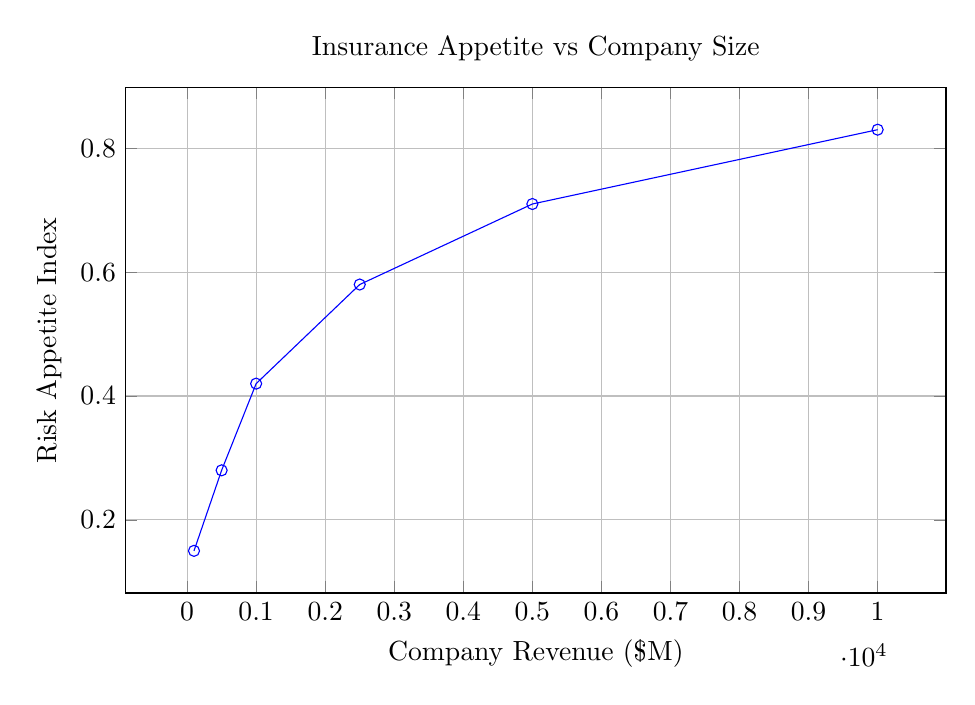
\begin{tikzpicture}
\begin{axis}[
    xlabel={Company Revenue (\$M)},
    ylabel={Risk Appetite Index},
    title={Insurance Appetite vs Company Size},
    grid=major,
    width=12cm,
    height=8cm
]
% Placeholder data - replace with actual results
\addplot[blue, mark=o] coordinates {
    (100, 0.15)
    (500, 0.28)
    (1000, 0.42)
    (2500, 0.58)
    (5000, 0.71)
    (10000, 0.83)
};
\end{axis}
\end{tikzpicture}
\caption{Risk appetite increases with company size (simulated results)}
\label{fig:appetite_vs_size}
\end{figure}

Figure \ref{fig:appetite_vs_size} demonstrates the positive correlation between company size and risk appetite, consistent with ergodicity economics predictions.

\subsection{Sensitivity Analysis}

% TODO: Present sensitivity analysis results

\section{Industry Implications}

\subsection{Applications for Underwriting and Pricing}

The simulation framework provides several practical applications:
\begin{itemize}
    \item Dynamic pricing models that account for company size effects
    \item Portfolio optimization considering temporal risk dynamics
    \item Competitive positioning analysis
\end{itemize}

\subsection{Portfolio Management Considerations}

% TODO: Discuss portfolio management implications

\subsection{Regulatory and Capital Allocation Insights}

% TODO: Discuss regulatory implications

\section{Future Research Directions}

\subsection{Framework Extensions and Enhancements}

Potential areas for future development include:
\begin{itemize}
    \item Integration with catastrophe modeling
    \item Multi-line portfolio effects
    \item Reinsurance optimization
\end{itemize}

\subsection{Additional Applications in P\&C Insurance}

% TODO: Outline future applications

\subsection{Industry Collaboration Opportunities}

% TODO: Discuss collaboration possibilities

\section{Conclusion}

This white paper has introduced a novel simulation framework based on ergodicity economics principles for analyzing insurance risk appetite. Our key findings demonstrate that company size significantly influences risk appetite, with larger insurers exhibiting greater willingness to underwrite risk. This finding has important implications for competitive dynamics and market structure in P\&C insurance.

The simulation framework provides a powerful tool for:
\begin{itemize}
    \item Understanding temporal risk dynamics
    \item Optimizing portfolio decisions
    \item Informing strategic planning
\end{itemize}

I encourage industry practitioners to explore these concepts further and welcome collaboration on extending this research.

The framework will provide new insights for companies making insurance decisions and is intended to answer questions such as "what is the ROI of our insurance program?", "how much insurance do we need?" and considerations of optimal insurance deductibles and limits.

% Bibliography
\bibliographystyle{apalike}
\bibliography{references}

% Appendices
\appendix
\section{Technical Appendix}

\subsection{Simulation Algorithm Details}

% TODO: Provide detailed algorithm descriptions

\subsection{Parameter Estimation Methods}

% TODO: Describe statistical methods used

\subsection{Code Repository}

The simulation framework code is available at:\\
\url{https://github.com/AlexFiliakov/Ergodic-Insurance-Limits}

\end{document}
